\chapter{Univariate analysis}
\label{ch:univariate-analysis}

\begin{definition}[Descriptive statistics]
  Descriptive statistics\index{descriptive statistics} are techniques that quantitatively describe or summarise features of a collection of information.
\end{definition}

\section{Example: super heroes}

In a study on super heroes, researchers are interested in several properties. 

\begin{itemize}
  \item How tall are they (See Figure~\ref{fig:heroes-size})?
  \item How safe are they making their community (See Table~\ref{tab:heroes-saves})?
  \item \ldots
\end{itemize}

We'll use this case throughout the chapter as an example.

\begin{figure}
  \centering
  \begin{tikzpicture}[xscale=4,yscale=2]
  \draw (0,2) -- (0,0);
  \foreach \num/\label in {0/0, 0.2/20, .4/40, .6/60, .8/80, 1/100, 1.2/120, 1.4/140, 1.6/160, 1.8/180, 2/200}{%
    \draw (0, \num) -- (2.5, \num);
    \draw[shift={(0, \num)}] (1pt,0pt) -- (-1pt,0pt) node[left] {\scriptsize \label};
  }
  
  \node[anchor=north] (hero1) at (0.3,1.5)
  {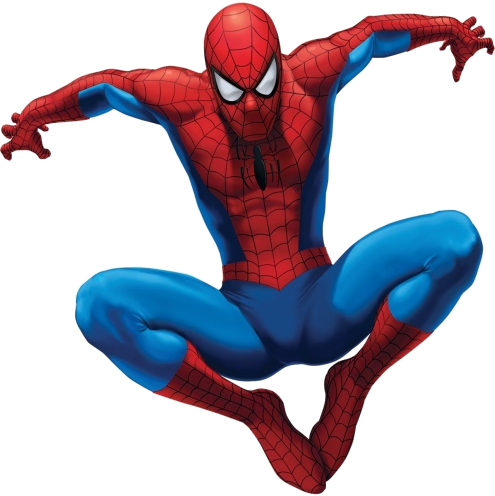
\includegraphics[height=2.9cm]{les2-hero-1}};
  \node[anchor=north] (hero2) at (0.8,2.05)
  {
\includegraphics[height=4cm]{les2-hero-2}};
  \node[anchor=north] (hero3) at (1.3,1.575)
  {
\includegraphics[height=3.1cm]{les2-hero-3}};
  \node[anchor=north] (hero4) at (1.8,2.1)
  {
\includegraphics[height=4.1cm]{les2-hero-4}};
  \node[anchor=north] (hero5) at (2.3,1.95)
  {
\includegraphics[height=3.8cm]{les2-hero-5}};
  
  \node (size1) at (0.3, 1.5) {\scriptsize 141 cm};
  \node (size2) at (0.8, 2.1) {\scriptsize 198 cm};
  \node (size3) at (1.3, 1.51) {\scriptsize 143 cm};
  \node (size4) at (1.8, 2.15) {\scriptsize 201 cm};
  \node (size5) at (2.3, 1.95) {\scriptsize 184 cm};
  \end{tikzpicture}
  
  \begin{tabular}{|c|c|c|c|c|}
    \hline
    $x_{1}$ & $x_{2}$ & $x_{3}$ & $x_{4}$&  $x_{5}$ \\
    \hline
    141 & 198 & 143 & 201 & 184 \\
    \hline
  \end{tabular}

  \caption{Superhero sizes, in cm.}
  \label{fig:heroes-size}
\end{figure}

\begin{table}
  
  \begin{center}
      
\includegraphics[width=.6cm]{les2-hero-2}
    \begin{tabular}{|c|c|c|c|c|c|c|c|}
      \hline
      4 & 7 & 11 & 16 & 20 & 22 & 25 & 26 \\
      \hline
    \end{tabular}
  
    
\includegraphics[width=.7cm]{les2-hero-3}
    \begin{tabular}{|c|c|c|c|c|c|c|c|c|c|c|c|c|c|c|}
      \hline
      3&7&5&13&20&23&39&23&40&23&14&12&56&23&29\\
      \hline
    \end{tabular}
  \end{center}
  
  \caption{The number of people saved during the last few years by Batman and Superman, respectively.}
  \label{tab:heroes-saves}
\end{table}

\section{Measures of central tendency}
\label{sec:measures-of-central-tendency}

\subsection{Arithmetic mean}
\label{ssec:arithmetic-mean}

\begin{definition}[Arithmetic mean]
  The \emph{arithmetic mean}\index{mean, arithmetic} or \emph{average} (notation $\overline{x}$, x-bar) of a set of values is the sum of all values divided by the number of values.
  \begin{equation}
    \overline{x} = \frac{1}{n} \times \sum_{i=1}^{n} x_{i}
    \label{eq:Mean}
  \end{equation}

  With:
  \begin{itemize}
    \item $x_{i}$ are the values of a set $X$,
    \item $n$ is the number of values in $X$.
  \end{itemize}
\end{definition}

\begin{exercise}
  What is the average length of the super heroes in Figure~\ref{fig:heroes-size}?
\end{exercise}

\begin{exercise}
  The average of 15 numbers is 12. Which number do we need to add to the row of numbers to get an average of 13?
\end{exercise}

The arithmetic mean is sensitive to outliers, i.e.~values far away from the mean. Extreme values can heavily influence the arithmetic mean.

\subsection{Median}
\label{ssec:median}

\begin{definition}[Median]
  The \emph{median}\index{median} is the value separating the higher half of a data set from the lower half.
\end{definition}

When you sort the values from low to high, the median will be the value in the middle. If the set has an even number of values, the median is the average of the two values in the middle. The median is much less sensitive to outliers.

\subsection{Mode}
\label{ssec:mode}

\begin{definition}[Mode]
  The \emph{mode} is the value that appears most often in a data set.
\end{definition}

The mode is pretty much useless in a data set where all or most values are unique. In that case, it's useful to subdivide the values in groups, each containing similar values. A dataset is called bimodal\index{bimodal} if it has two modes, and multimodal\index{multimodal}.

\begin{example}
  The data set with the number of people saved by Batman during the last eight years (see Table~\ref{tab:heroes-saves}) could be subdivided as follows:
  
  \begin{itemize}
    \item $[0-9]$ people: 4, 7
    \item $[10-19]$ people: 11, 16
    \item $[20-29]$ people: 20, 22, 25, 26
    \item $[30-39]$ people: 33
  \end{itemize}
  
  Category $[20-29]$ occurs the most, and is called the \emph{modal class}. We could use the center of this range, i.e.~25, as the mode.
\end{example}

\section{Measures of dispersion}
\label{sec:measures-of-dispersion}

\subsection{Variance and standard deviation}
\label{ssec:variance-and-standard-deviation}

\begin{definition}[Variance]
  The \emph{variance}\index{variance} (notation: $\sigma^{2}$, sigma squared) is the mean squared difference between the values of a data set and the arithmetic mean.
  \begin{equation}
  \sigma^{2} = \frac{1}{n} \times \sum_{i=1}^{n} \left( \overline{x} - x_i \right)^{2}
  \label{eq:variance}
  \end{equation}
\end{definition}

The variance of a data set will be 0 if and only if all values are exactly equal.

\begin{example}
  The variance of the lengths of our super heroes is calculated as follows:
  
  \begin{equation}
  \begin{aligned}
  \sigma^{2} &= \frac{(173.4-141)^{2} + (173.4 - 198 )^{2} + (173.4 - 143)^{2} + (173.4- 201)^{2} + (173.4 - 184 )^{2}}{5} \\
             &= \frac{(-32.4)^{2} + (24.6)^{2} + (-30.4)^{2}+ (27.6)^{2} + (10.6)^{2}}{5}\\
             &= \frac{1049.76 + 605.16 + 924.16 + 761.76 + 112.36}{5}\\
             &= \frac{3453.2}{5} = 690.64
  \end{aligned}
  \end{equation}
\end{example}

\begin{definition}[Standard deviation]
  The \emph{standard deviation}\index{deviation, standard}\index{standard deviation} is the square root of the variance.
  \begin{equation}
  \sigma = \sqrt{\sigma^{2}}
  \label{eq:stdev}
  \end{equation}
\end{definition}

The standard deviation is one of the most often used measures of dispersion. A small standard deviation indicates that the values are close to the arithmetic mean ($\overline{x}$), a large standard deviation that the values are dispersed over a larger range of values. In some cases, a small standard deviation is desired, in other cases, it may not be that important.

\begin{example}
  In the manufacturing process of screw drivers, the size of the head is important for its functioning. When the heads of a batch of 1000 screw drivers is measured, their sizes should be the same, so a very small standard deviation is an indication of good quality.
\end{example}

\begin{example}
  Super heroes are a very diverse group. Some are very rich (e.g.~Batman, Iron Man), some are middle class (e.g.~Spiderman), others are quite poor (e.g.~Arsenal). The dispersion of their income would be very large, but that isn't necessarily a bad thing.
\end{example}

An interesting property of the standard deviation is that it is expressed in the same unit as the measured date. In the example of the size of super heroes, the standard deviation is 26.28 cm. Just like the arithmetic mean, the variance and standard deviation are sensitive to outliers. The variance is even more sensitive than the mean, because of the squared differences.

\subsection{Range}
\label{ssec:range}

\begin{definition}[Range]
  The \emph{range}\index{range} of a data set is the absolute value of the difference between the highest and the lowest value.
\end{definition}

\subsection{Quartiles}
\label{ssec:quartiles}

\begin{definition}[Quartiles]
  The \emph{quartiles}\index{quartiles} of a sorted set of numbers are the three values that divide the set into 4 equally large subsets.

  \begin{itemize}
    \item the first/lower quartile ($Q_{1}$) is the value that separates the lowest quarter of values from the rest
    \item the second quartile ($Q_{2}$) is the value that separates the lowest half of values from the highest half.
    \item the third/higher quartile ($Q_{3}$) is the value that separates the highest quarter of values from the rest
  \end{itemize}
\end{definition}

\begin{exercise}
  \label{ex:q2}
  The second quartile, $Q_2$ corresponds with which statistic discussed in this chapter?
\end{exercise}

The concept of quartiles can be generalised to percentages. The $P$-th \emph{percentile} of a list of ordered values is the smallest value in the list such that $P$ percent of the data is less than or equal to that value.

\begin{definition}[Interquartile range]
  The \emph{interquartile range}\index{range, interquartile} (IQR) is the difference between the higher and lower quartile.
  \begin{equation}
    \mathrm{IQR} = Q_3 - Q_1
    \label{eq:iqr@}
  \end{equation}
\end{definition}

If $n$ is an odd number, then~\autocite{Moore2002}:
\begin{itemize}
  \item $Q_{1}$ is the $\frac{n+1}{4}$'th value;
  \item $Q_{3}$ is the $\frac{3n+3}{4}$'th value.
\end{itemize}

If $n$ is an even number, however:
\begin{itemize}
  \item $Q_{1}$ is the $\frac{n+2}{4}$'th value;
  \item $Q_{3}$ is the $\frac{3n+2}{4}$'th value.
\end{itemize}

\section{Application to levels of measurement}
\label{sec:application-to-levels-of-measurement}

The measures of centrality and dispersion discussed previously are each suited for variables with a specific level of measurement. This is summarised in Table~\ref{tab:levels-of-measurement}.

\begin{table}
  \centering
  \begin{tabular}{|l|l|l|l|}
  	\hline
  	\textbf{Measure of} & \textbf{Nominal} & \textbf{Ordinal}    & \textbf{Interval}, \textbf{Ratio} \\ \hline
  	\textbf{Centrality} & Mode             & Median              & Mean                              \\
  	                    & Modal class      & Mode                & Median                            \\
  	                    &                  & Modal class         & Modal class                       \\ \hline
  	\textbf{Dispersion} &                  & Range               & Standard deviation                \\
  	                    &                  & Interquartile range & Interquartile range               \\
  	                    &                  &                     & Range                             \\ \hline
  \end{tabular}
  \caption{Summary of which measures of centrality or dispersion are suitable for which levels of measurement.}
  \label{tab:levels-of-measurement}
\end{table}

\section{Charts}
\label{sec:charts}

\subsection{Boxplot}
\label{ssec:boxplot}

A boxplot\index{boxplot} is a chart that shows the dispersion of a set of values (see Figure~\ref{fig:boxplot}). It is formed by a rectangle with sides at the quartiles ($Q_1$ and $Q_3$). Inside the rectangle, the median is drawn as well. The whiskers attached to the upper and lower sides of the rectangle cover the rest of the observations, excepting outliers and extremes.

\begin{itemize}
  \item An \emph{outlier}\index{outlier} is a value that is more than 1.5 times the IQR below the lower quartile or above the higher quartile. It is indicated with a circle.
  \item An \emph{extreme value}\index{extreme} is a value that is more than 3 times the IQR below the lower quartile or above the higher quartile. It is indicated with a star.
\end{itemize}

\begin{figure}
  \centering
  % Source: http://mirrors.ibiblio.org/CTAN/graphics/pgf/contrib/pgfplots/doc/pgfplots.pdf
  % p.430
  \begin{tikzpicture}
  \begin{axis}[x=3cm,xticklabels={},xmax=2.3]
  \addplot+[
  boxplot prepared={
    draw direction=y,
    lower whisker=5,
    lower quartile=7,
    median=8.5,
    upper quartile=9.5,
    upper whisker=10,
  },
  ]
  table[row sep=\\,y index=0] {
    data\\ 1\\ 3\\
  }
  [right,color=HoGentAccent2]
  node at
  (boxplot box cs: 1,.6)
  {outlier}
  node at
  (boxplot box cs: \boxplotvalue{lower quartile},1)
  {$Q_1$}
  node at
  (boxplot box cs: \boxplotvalue{median},1)
  {$Q_2$, median}
  node at
  (boxplot box cs: \boxplotvalue{upper quartile},1)
  {$Q_3$}
  node at
  (boxplot box cs: \boxplotvalue{upper whisker},1)
  {max}
  ;
  \end{axis}
  \end{tikzpicture}
  
  
  \caption{Example of a boxplot.}
  \label{fig:boxplot}
\end{figure}

\section{Exercises}
\label{sec:exercises-univariate-analysis}

\subsection{Univariate statistics}

\begin{definition}[Frequency table]
  A \emph{frequency table}\index{frequency table} is a table that summerises how often each value occurs in the data set.
\end{definition}

\begin{exercise}
  How should the formulas for variance (Equation~\ref{eq:variance}) and standard deviation (Equation~\ref{eq:stdev}) be adapted in order to be usable with a frequency table? Apply these formulas to the data in Table~\ref{tab:pinfreq}.
\end{exercise}

\begin{table}
  \centering
  \begin{tabular}{@{}ll@{}}
    \toprule
    Pins $x$ & Frequence $f_{x}$ \\ \midrule
    0        & 2                 \\
    1        & 1                 \\
    2        & 2                 \\
    3        & 0                 \\
    4        & 2                 \\
    5        & 4                 \\
    6        & 9                 \\
    7        & 11                \\
    8        & 13                \\
    9        & 8                 \\
    10       & 8                 \\ \bottomrule
  \end{tabular}
  \caption{Frequency table for the number of pins knocked down in a game of bowling.}
  \label{tab:pinfreq}
\end{table}

\begin{exercise}
  \label{ex:variance-formula}
  Why does variance (see Equation~\ref{eq:variance}) use the square of the difference? Why not the numbers themselves (i.e. $(\overline{x} - x_i)$) or the absolute value of the difference (i.e. $\left|\overline{x} - x_i\right|$)?
  
  \[ \sigma^{2}_{1} = \frac{1}{n} \sum_{i=1}^{n} (\mu - x) \]
  \[ \sigma^{2}_{2} = \frac{1}{n} \sum_{i=1}^{n} \left| \mu - x\right| \]
  \[ \sigma^{2}_{3} = \frac{1}{n} \sum_{i=1}^{n} (\mu - x)^{2} \]
  
  Try out each variant of the equation with the data sets $X = \left\{4,4,-4,-4\right\}$ and $Y = \left\{7,1,-6,-2\right\}$.
\end{exercise}

\begin{exercise}
  Look up what the \emph{coefficient of variation} (CV) means. How is it defined? What is the major difference with the standard deviation?
\end{exercise}

\begin{exercise}
  In the following exercises, we're going to use the experimental results from~\textcite{Akin2016}. These are stored in the file \texttt{android\_persistence\_cpu.csv}.

  Open this file in a spreadsheet application and study the structure of the data. Can you identify the variables and their level of measurement?

  We will be using the \texttt{R} programming language for statistical computing with RStudio\footnote{\url{https://www.rstudio.com/}}. Start RStudio and create a new R script. Save it into the same directory as the data file. In the menu, select Session > Set Working Directory > To source file location. Enter the following line of code:

\begin{lstlisting}
android_cpu <- read.csv("android_persistence_cpu.csv",
                        sep=";")
attach(android_cpu)
\end{lstlisting}

After loading the data, let's look at average time, standard deviation, quartiles, etc.~over the entire data set. Use the appropriate R functions: \texttt{mean}, \texttt{median}, \texttt{quantile}, \texttt{min}, \texttt{max}, \texttt{var}, \texttt{sd}.

Tips:

\begin{itemize}
  \item A column/variable of a data table is referred to as: \verb|Table$Column|. When you have \verb|attach|ed the table, you can use the \verb|Column| name directly.
  \item You can group values according to a qualitative value with \verb|Variable ~ Categories|.
\end{itemize}
\end{exercise}

\begin{exercise}
Is it possible to draw conclusions from these results? If so, what are they? If not, why not?
\end{exercise}

\subsection{Charts in R}
\subsubsection{Histogram}

A histogram is a plot that shows the frequencies of observations between specific ranges.

\begin{lstlisting}
hist(android_cpu$Time, main="Distribution of execution time",
     xlab="Execution time")
hist(android_cpu$Time, main="Distribution of execution time",
     xlab="Execution time", breaks=2)
\end{lstlisting}

\begin{exercise}
Generate a histogram for \texttt{android\_cpu\$Time}\footnote{You can find general info about generating plots in R here:  \url{https://www.datacamp.com/community/tutorials/15-questions-about-r-plots\#gs.RK_ORsI}.}.
 
Can you draw useful conclusions from this graph? What happens if you increase the number of \texttt{breaks}?
\end{exercise}

\subsubsection{Boxplot}

A boxplot shows the median, quartiles, and extremes in a dataset. It gives a good impression of the distribution of the data.

\begin{lstlisting}
boxplot(android_cpu$Time)
boxplot(android_cpu$Time, main='Distribution of CPU time',
        ylab='Time in ms');
\end{lstlisting} 

\begin{exercise}
  By default, boxplots are drawn vertically. Use the help function in RStudio to find out how to draw it horizontally.
\end{exercise}

In the previous exercises, when we tried to analyse the dataset as a whole, we noticed that this is pretty much useless, since the data set is divided into several categories. Let's create boxplots for each category.

\begin{lstlisting}
boxplot(android_cpu$Time ~ android_cpu$DataSize,
        main='Distribution of CPU time over data sizes',
        ylab='Time in ms');
\end{lstlisting}

\begin{exercise}
\label{ex:boxplot}
Interpret the results from this plot. Do these make more sense?
\end{exercise}

We kunnen hetzelfde doen voor de verschillende soorten dataopslagmogelijkheden in android.

\begin{exercise}
  Do the same as in \ref{ex:boxplot}, but group by \verb|PersistenceType| and interpret the results. Do these make sense?
\end{exercise}

Finally, let's see how the data is distributed over \emph{both} categories.

\begin{lstlisting}
boxplot(android_cpu$Time ~ android_cpu$PersistenceType * android_cpu$DataSize)
\end{lstlisting}

By looking at the data over the different categories, we get a clearer view on the data, but the graph is a bit overcrowded now.

There are several ways of selecting data that meets specific criteria, a.o.~the functions \verb|which| and \verb|subset|.

\begin{lstlisting}
greenDOA <- android_cpu[which(android_cpu$PersistenceType=='GreenDAO'),]
boxplot(greenDOA$Time~greenDOA$DataSize)
\end{lstlisting}

\begin{exercise}
Wat can you conclude from this plot?
\end{exercise}

\begin{exercise}
Find out which box plots are meaningful for this data and whether your results match those of~\textcite{Akin2016}. What are your conclusions?
\end{exercise}



\section{Solutions to selected exercises}

Exercise~\ref{ex:q2}: the median

Exercise~\ref{ex:variance-formula}:

\begin{itemize}
  \item When using the values themselves, negative and positive values would cancel out each other, resulting in a variance of 0 in set $X$.
  \item When using the absolute value, both data sets would have the same variance, although the dispersion of set $Y$ is clearly larger.
  \item When squaring the differences, these problems do not occur.
\end{itemize}
